\documentclass{beamer}

\title{Summer 2025}
\author{Aatu Selkee}
\date{June 10, 2025}


\usepackage{subfigure}

\begin{document}

\frame{\titlepage}


\begin{frame}{Main research topics}
    \begin{itemize}
        \item Bayesian optimization
        \item Time series analysis
        \begin{itemize}
            \item Two different problems, one with less datapoints and a known underlying structure, another with about 100 000 datapoints.
        \end{itemize}
        \item Gaussian processes
        \begin{itemize}
            \item Slight variations of the standard Gaussian process regression model.
            \item Deep kernel learning and deep Gaussian processes.
        \end{itemize}
    \end{itemize}
\end{frame}

\begin{frame}{Gaussian processes}
    \begin{figure}
        \centering
        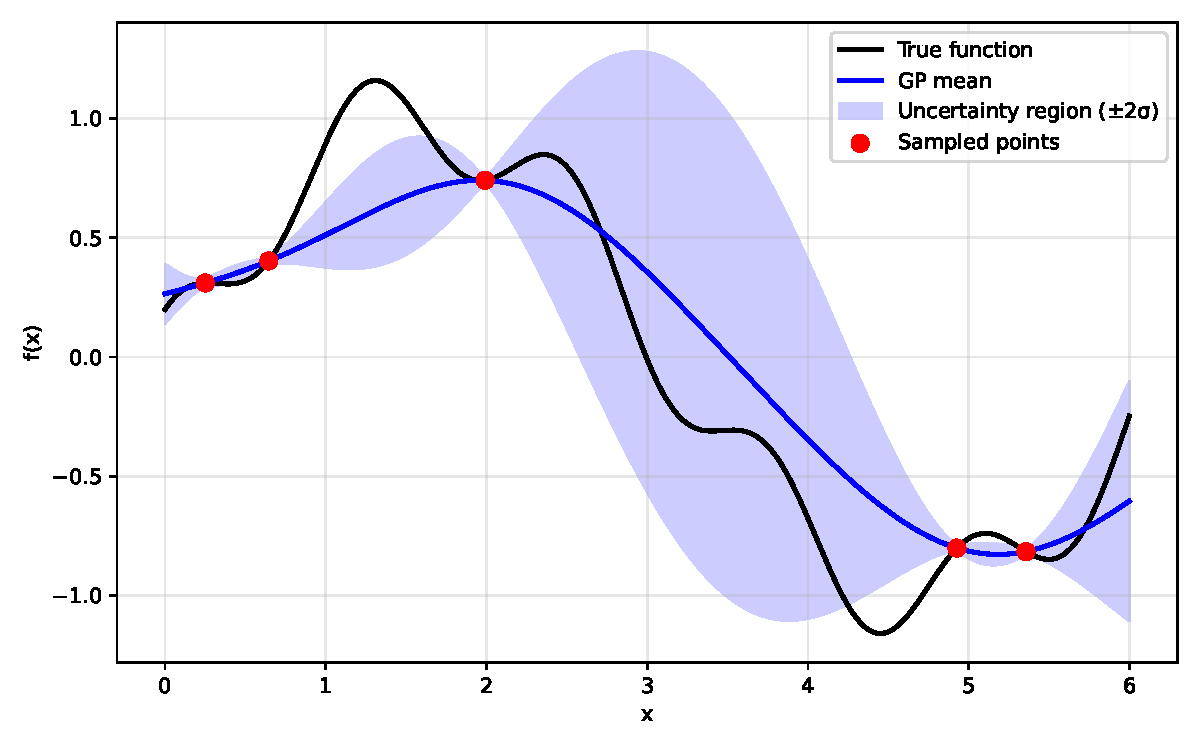
\includegraphics[width=\textwidth]{./July presentation/sausage_plot.pdf}
        \caption{Plot of a Gaussian process approximating a known function with 5 samples.}
    \end{figure}
\end{frame}

\begin{frame}{Bayesian optimization}
    \begin{figure}
        \begin{subfigure}
            \centering
            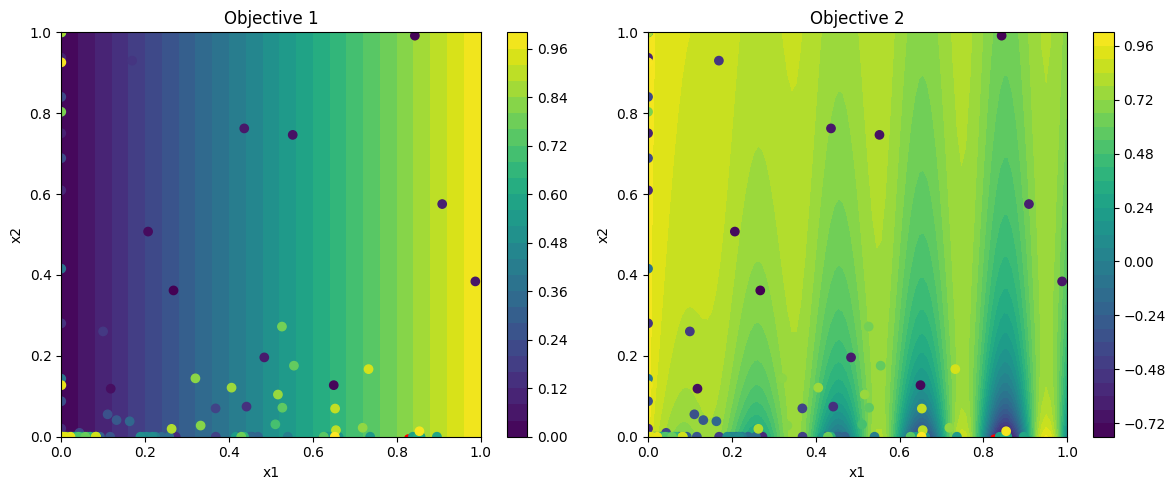
\includegraphics[width=0.9\textwidth]{../Images/DeepKernelLearning/DKL_result_X.png}
        \end{subfigure}
        \begin{subfigure}
            \centering
            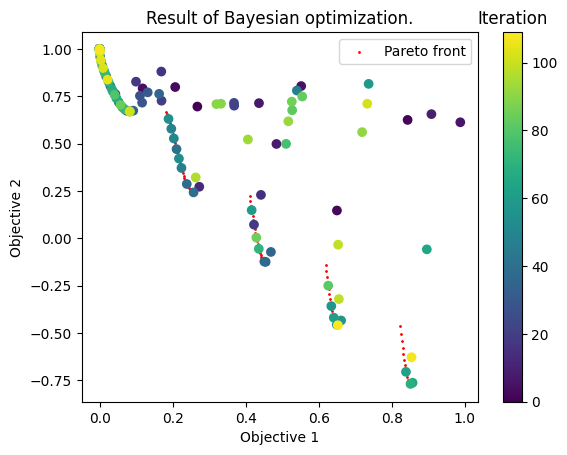
\includegraphics[width=0.5\textwidth]{../Images/DeepKernelLearning/DKL_result_Y.png}
        \end{subfigure}
    \end{figure}
\end{frame}


\end{document}